\documentclass{article}

\usepackage{listings}
\usepackage{amssymb}
\usepackage{geometry}
\usepackage{xcolor}
\usepackage{graphicx}
\geometry{margin=1in}


\begin{document}


\begin{center}


\includegraphics[width = 3cm ]{matcom.jpg.jpeg}
\Huge \em 
\textcolor {black}{Proyecto Moogle}

\huge \textcolor {black} {Melani Forsythe , curso : 2022 - 2023 } 

\vspace{0.5cm}

\end{center}

\Large \textcolor {blue}{INTRODUCCION}

\vspace{0.5cm}

Moogle es una aplicacion cuyo proposito es buscar un texto en un conjunto de documentos .Para ello usamos el Modelo de recuperacion Vectorial ,en el cual a traves de las palabras presentes en cada documento y sus pesos ,logramos crear un vector por documento y aplicar la similitud cosenica con el vector relativo a la consulta , de esta forma se obtiene un ranking donde el resultado mas elevado sera el documento con mas similitud a la consulta hecha ,es decir el mas recomendado de acuerdo a la busqueda del usuario.
\vspace{1.0cm}

\Large \textcolor{blue}{ DESARROLLO}

\vspace{0.5cm}

En su arquitectura cuenta con varias clases como por ejemplo :
\vspace {0.5cm }

\large \textcolor {blue}{CLASE PROCESAMIENTO DEL CORPUS }:

\vspace {0.3cm}

Esta clase lee la direccion dada y busca entre las carpetas y subcarpetas y lee el contenido en ellas,
Obtiene el nombre de cada docuemnto y despues de haber leido cada uno les retira los caracteres raros y los signos de puntuacion ,lo mismo pasa con el query.

\vspace{0.5cm}

\large \textcolor {blue}{CLASE SCORE}: 

\vspace {0.3cm}
Esta clase se encarga de los calculos del programa ,primero obtiene el vocabulario del corpus  y los introduce en un diccionario 
Cuenta con un metodo llamado VECTORS el cual calcula el TFIDF al query.
\tiny
\begin{lstlisting}

    public static  Dictionary <string,Dictionary<string , double >> vectors(string query ,string [] docs, string [] name )
 {
    List <string> cadena = new List<string>(){query};
    cadena = query.Split(' ').ToList();
    Dictionary <string , double > TFIDF= new Dictionary<string , double >();
    Dictionary <string ,Dictionary<string, double >> vector = new Dictionary<string ,Dictionary<string , double >>();

      for (int k = 0; k < docs.Length; k++)
      {
         TFIDF = dicc(query,docs[k],docs);

         vector.Add(name [k],TFIDF);
        
      }
       return vector;
 }
\end{lstlisting}

\vspace{1.0 cm}
\large
El TF-IDF es una estadistica numerica que se utiliza para describir una de las formas en  q un  motor de busqueda puede determinar si un texto es relevante en relacion con los terminos utilizados en una consulta de busqueda .El TF – IDF se calcula multiplicando la frecuencia de los terminos por la frecuencia de documento inversa 
\vspace{1.0cm}

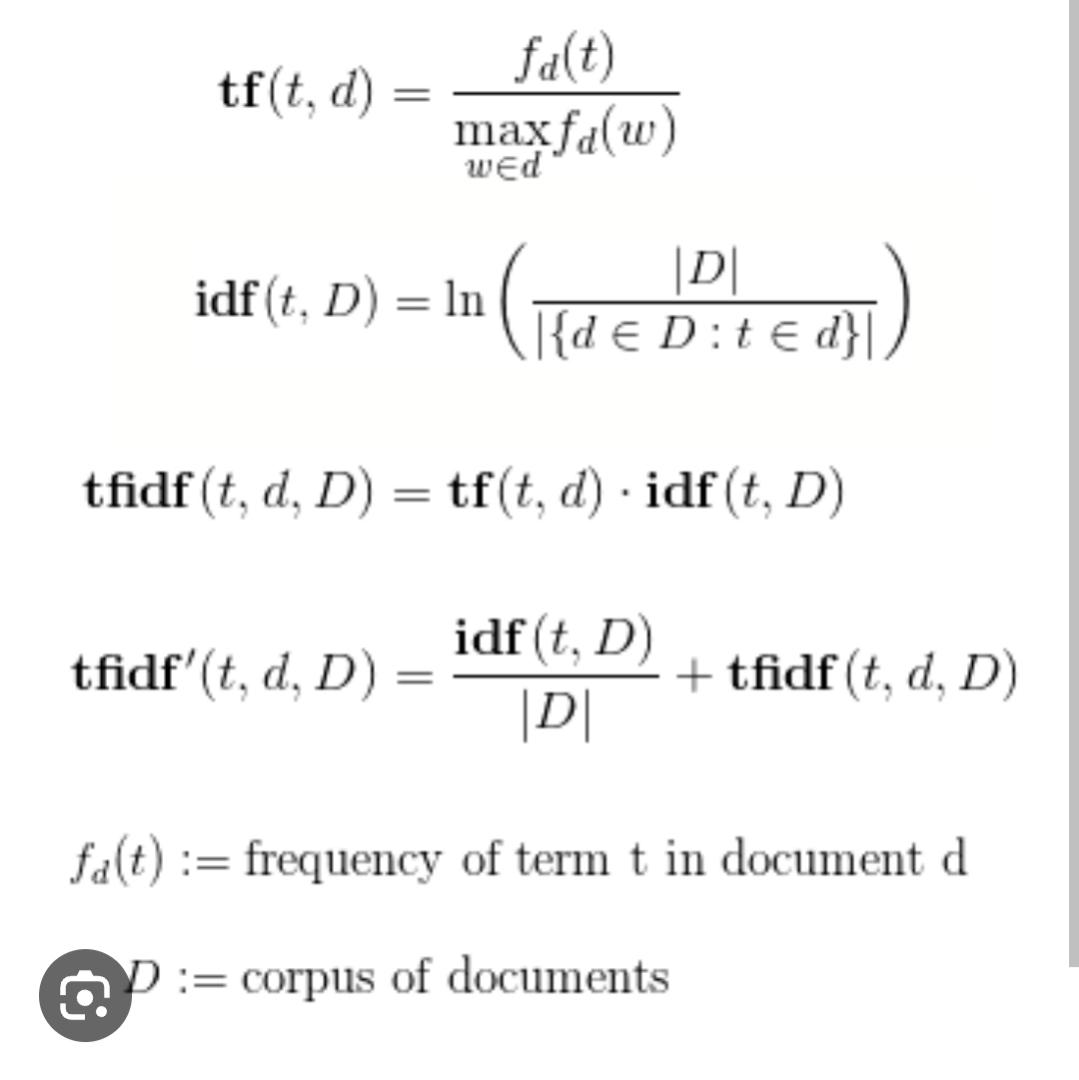
\includegraphics[width=10cm]{tf-idf.jpg.jpeg}

\vspace{0.2cm}

Tambien cuenta con el metodo de similitud cosenica ,es una medida que se utiliza para calcular la similitud entre dos o mas vectores . La similitud del cosena del angulo entre vectores .Los vectores suelen ser distintos a cero y estan dentro de un espacio de producto escalar .
En terminos matematicos la similitud del coseno se describe como la division entre el producto escalar de los vectores y el producto de las normas euclideanas o la magnitud de cada vector .

\vspace{0.2cm}
\textcolor{blue}{ Metodo de similitud cosenica }:
\small
\begin{lstlisting}
    
    public  static  double  CalSimilitudCos( double  [] query ,  double  [] documento)
    {
           double  producto = PRODUCTO(query,documento);
          
           double  magnitudA = MAGNITUD(documento);
          
           double  magnitudB = MAGNITUD(query);
        
           double  prod =  producto /magnitudA*magnitudB  ;
          
          return prod;
  
    }
\end{lstlisting}

\large \textcolor {blue}{CLASE METODOS AUXILIARES} :

\vspace{0.2cm}

Esta clase contiene al metodo ESCOREANDO que nos devuelve el escore según los calculos de los valores de las palabras ,tambien nos modifca el escore según la utilizacion de los operadores de busqueda
En este clase  tambien se obtiene el snippet de cada docuemnto se basa en obtener la palabra mas relevante de la query y a partir de ella coger 400 caracteres hacia adelante .

\vspace{0.5cm}

\large\textcolor {blue} {CLASE OPERADORES}

\vspace{0.2cm}

En esta clase los metodos mas importantes son MODIFICAR y VALOR modificar se encarga de asegurarse que los operadores de excluion y inclusion no se encuentren y en caso de no encontrarlos y la consulta tener alguno de los dos operadores restantes llama al metodo VALOR y modifica el escore según los operadores.

\vspace{0.5cm}

\large \textcolor {blue} {CLASE MOOGLE}

\vspace{0.2cm}

Este metodo es la recta final aquí declaro todas las variables a usar para retornar finalmente el documento deseado.
Observaciones: Este programa puede ser sujeto a cambios para mejorar su rendimiento asi como el cambio de la interfaz ,la reformulacion del codigo para hacerlo mas compacto y eficiente.

\vspace{1.0 cm }

\large \textcolor {blue}{MODO DE USO} 

\vspace{0.5cm}

Para facilitar la busqueda hemos implementado operadores de busqueda tales como inclusion ,exclusion , mayor relavancia y cercania 

\textcolor {green} {OPERADORES}
\vspace{0.2cm}

\textbf {Exclusion} :indentificado con un " ! " delante de la palabra "ej,!melani" indica que la palabra no debe aparecer en ningun documento devuelto.

\vspace{0.2cm}

\textbf {Mayor relevancia }: indentificado con un " * "delante de la palabra " ej,*melani ". la relevancia en donde aparezca esta palabra se multiplica por la cantidad de asteriso por 5 .

\vspace{0.2cm}

\textbf {Cercania} : indentificado con un " ~ " entre las palabras ,usando la tecla de espacio entre ellas y solo una vez por consulta " ej,melani ~ forsythe " indica que los docuemntos que tenga la menor distancia entre estas dos palabres tendran mayor puntuacion. (\textbf{solo usar un " ~ " de lo contrario no funcionara})

\vspace{0.5cm}

\Large \textcolor {blue} {SUGERENCIA}

\vspace{0.5cm}

Le brinda al usuario una palabra  de la base de datos parecida a la ingresada .
Para la implementacion de esta funcion se utilizo distancia de Levenshtein .Esta funcion es una metrica de cadenas para medir la diferencia entre dos secuencias .De manera informal , la distancia de Leveshtein  entre dos palabras es el numero minimo de ediciones de un solo carácter necesaras para cambiar una palabra por otras .
\small
\begin{lstlisting}

   public static int levenshteinDistance(string salida , string llegada)
   {
     int distancia = int.MaxValue;
 LD(salida , llegada ,salida.Length-1,llegada.Length - 1,ref distancia ,0);
 return distancia;

 void LD(string s , string l ,int i ,int j , ref int mejor_distancia , int distancia_acum)
 {
  if(distancia_acum >= mejor_distancia || distancia_acum >= s.Length/2)return;
   if (i==-1)
   {
     mejor_distancia = Math.Min(distancia_acum + j + 1,mejor_distancia);return ;};
     if (j== -1)
     {
       mejor_distancia = Math.Min(distancia + i + 1,mejor_distancia); return ;};
     
     if (s[i] ==l[j])
     {
       LD(s, l ,i-1,j -1,ref mejor_distancia,distancia_acum);return ;}
       else
       {
         distancia_acum+=1;
         LD(s,l,i-1,j-1,ref mejor_distancia,distancia_acum);
         LD(s,l,i,j-1,ref mejor_distancia,distancia_acum);
         LD(s,l,i-1,j,ref mejor_distancia,distancia_acum);
      }
   }

   }
   
\end{lstlisting}

\end{document}